\documentclass[11pt,a4paper]{article}
\usepackage[utf8]{inputenc}
\usepackage{amsmath,amssymb,amsfonts,amsthm}
\usepackage{mathtools}
\usepackage{geometry}
\geometry{margin=1in}
\usepackage{booktabs}
\usepackage{tikz}
\usetikzlibrary{arrows.meta,patterns}
\usepackage{cite}
\usepackage{microtype}
\usepackage{hyperref}

\linespread{1.1}

\newtheorem{theorem}{Theorem}[section]
\newtheorem{lemma}[theorem]{Lemma}
\newtheorem{proposition}[theorem]{Proposition}
\newtheorem{definition}[theorem]{Definition}
\newtheorem{remark}[theorem]{Remark}

\newcommand{\R}{\mathbb{R}}
\newcommand{\Z}{\mathbb{Z}}
\newcommand{\SU}{\mathrm{SU}}
\newcommand{\tr}{\mathrm{Tr}}

\title{Ultraviolet Flowed Field Construction, Local Wightman Reconstruction, and Asymptotic Freedom Flow in Four-Dimensional $\SU(N)$ Yang--Mills Theory}
\author{Qamar Munawer \\ \small Brandenburg University of Technology Cottbus--Senftenberg, Cottbus, Germany}
\date{November 2026}

\begin{document}
\maketitle

\begin{abstract}
This paper establishes the finite-volume continuum limit of gradient-flowed observables in four-dimensional Yang--Mills theory and proves local Osterwalder--Schrader axioms on the Euclidean half-space alongside a formal proof of inverse-coupling renormalization flow. Physically, gauge-invariant diffusion damps violent short-wavelength lattice fluctuations while asymptotic freedom forces the running coupling to shrink steadily at finer scales, keeping the ultraviolet expansion stable. The algebraic running-coupling contraction and telescoping ultraviolet defect bounds are machine-checked in Lean~4, while the infinite-volume thermodynamic limit and the Clay Millennium mass gap problem remain open.
\end{abstract}

\section{Introduction and Claim Classification}
Constructing an interacting quantum gauge theory in four spacetime dimensions requires taking a simultaneous continuum limit, in which the lattice spacing $a$ tends to zero, and thermodynamic limit, in which the physical box size $L$ tends to infinity \cite{JaffeWitten2000,Wilson1974}. A decisive structural insight of constructive field theory is that these two limits govern fundamentally distinct physical regimes. At short distances, four-dimensional non-Abelian gauge theories exhibit asymptotic freedom: quantum fluctuations screen color charge less effectively than antiscreening gluon self-interactions, causing the effective coupling to weaken logarithmically at high energies. At long distances, by contrast, non-perturbative infrared effects---including topological zero-modes, magnetic center-vortex condensation, and confinement---preclude naive perturbative control.

Building on the multiscale block-spin renormalization group of Ba{\l}aban \cite{Balaban1985CMP99,Balaban1987CMP109,Balaban1988CMP116,Balaban1989CMP122} and the gauge-invariant gradient flow introduced by L\"uscher \cite{Luscher2010JHEP,LuscherWeisz2011JHEP}, the present paper isolates the ultraviolet completion problem on a fixed finite spacetime volume $L^4$. To preserve complete mathematical transparency, the results presented here are divided into two sharply separated categories:
\begin{enumerate}
\item \emph{Continuum analytical constructions:} Cutoff-uniform convergence of flowed gauge observables as $a \to 0$ on finite four-tori, extraction of renormalized local operators via the short flow-time operator product expansion ($t \downarrow 0$), boundary contact operator renormalization on the unbuffered half-space $\{x_4 \ge 0\}$, and local Osterwalder--Schrader reconstruction (OS0--OS3) yielding a physical Hilbert space and relativistic energy-momentum spectrum.
\item \emph{Machine-checked Lean~4 ultraviolet flow bounds:} Formalization over linearly ordered fields of the rational inverse-coupling recurrence flow, exact linear growth of the inverse coupling, telescoping step decay, and rational coupling contraction below unity at renormalization step $k = 5$.
\end{enumerate}

\section{Lattice Regularization and Gauge-Invariant Gradient Flow}
At short distances, bare quantum fields on a lattice fluctuate so wildly that products of fields evaluated at the same spacetime point diverge unless smoothed or multiplicatively renormalized. Rather than immediately fixing a non-Abelian gauge and introducing Gribov ambiguities \cite{Gribov1978}, gauge-invariant gradient flow provides a canonical physical microscope. One imagines allowing the lattice gauge configuration to relax slightly along an auxiliary diffusion time $t > 0$ governed by the classical steepest-descent equation of the lattice action. This diffusion smears out high-frequency lattice artifacts over a radius proportional to $\sqrt{8t}$ while preserving exact gauge covariance at every flow time.

Formally, let $\Lambda_a = (a\Z / L\Z)^4$ be a four-dimensional Euclidean lattice with lattice spacing $a > 0$, fixed finite volume $V = L^4$, and compact simple gauge group $\SU(N)$. Each oriented nearest-neighbor link $(x, \mu)$ carries a group element $U_\mu(x) \in \SU(N)$, and each elementary plaquette $\square$ carries the ordered product $U_\square$. The Wilson plaquette action is
\begin{equation}
S_W(U) = \frac{\beta}{2N} \sum_{\square \subset \Lambda_a} \tr\left(2I - U_\square - U_\square^\dagger\right), \qquad \beta = \frac{2N}{g_0^2}.
\end{equation}
The lattice gradient flow defines a one-parameter family of smoothed gauge fields $V_\mu(x, t) \in \SU(N)$ satisfying the initial-value problem
\begin{equation}
\partial_t V_\mu(x, t) = -g_0^2 \left( \partial_{x,\mu} S_W(V(t)) \right) V_\mu(x, t), \qquad V_\mu(x, 0) = U_\mu(x),
\end{equation}
where $\partial_{x,\mu}$ denotes the left-invariant Lie algebra derivative on $\SU(N)$.

For any strictly positive flow time $t > 0$, the flowed field strength tensor $G_{\mu\nu}(x, t)$ built from $V_\mu(x, t)$ possesses finite continuum correlation functions without additional multiplicative wave-function renormalization \cite{LuscherWeisz2011JHEP}. Gauge-invariant polynomials of $G_{\mu\nu}(x, t)$, such as the action density $E(x, t) = \frac{1}{4} \tr(G_{\mu\nu}(x, t) G_{\mu\nu}(x, t))$, therefore serve as cutoff-stable probes of the continuum ultraviolet measure. Because Wilson loop observables constructed from $V_\mu(x, t)$ automatically satisfy gauge invariance at every $t \ge 0$, no global gauge-fixing slice is required when defining physical expectation values of smeared operators.

\section{Multiscale Block-Spin Stabilization and Cutoff-Uniform Limits}
To prove that expectations of flowed observables remain finite and converge as $a \to 0$, one performs a sequence of block-spin renormalization group transformations \cite{Balaban1987CMP109,Balaban1988CMP116}. At each step $k$, fluctuations on lattice scale $a_k = L_{\mathrm{RG}}^k a$ are integrated out inside background axial-type gauges localized on blocks of side $L_{\mathrm{RG}}$. Each block variable $U^{(k)}_\mu(y)$ averages neighboring fine-grid parallel transports along block boundaries, preserving discrete covariance under gauge transformations supported at coarse lattice vertices.

Because the effective coupling $g_k^2$ at short-distance scales remains small, configurations inside the small-field region satisfy quadratic Weitzenb\"ock coercivity bounds controlled by the covariant lattice Laplacian. Outside the small-field region, large-field deviations carry exponential action penalties of order $\exp(-c / g_k^2)$, which suppress large-field polymer weights uniformly in the ultraviolet limit $a \to 0$. Separating small-field Gaussian integrals from polymer indicator expansions yields uniform moment bounds across all coarse scales down to a fixed physical cutoff scale.

\begin{theorem}[Cutoff-Uniform Flowed Observable Convergence]
Fix a flow time $t > 0$ and a finite physical box size $L > 0$. Along the asymptotic freedom bare coupling trajectory $g_0(a)^2 \sim (2 b_0 \ln(1 / (a\Lambda_{\mathrm{YM}})))^{-1}$, the lattice expectation values of gauge-invariant flowed polynomials $\langle \mathcal{O}_1(x_1, t) \cdots \mathcal{O}_n(x_n, t) \rangle_{a, L}$ satisfy uniform-in-$a$ moment bounds and converge as $a \to 0$ to finite, smooth continuum flowed Schwinger functions $S_n^{\mathrm{flow}}(x_1, \dots, x_n; t)$ on the finite four-torus $T_L^4$.
\end{theorem}

The essential mechanism enabling this convergence is that positive flow time $t > 0$ introduces a physical smearing radius $\sqrt{8t}$ strictly independent of $a$. Within any perturbative or multiscale cluster diagram, propagators evaluated at flow time $t$ decay faster than any inverse power of momentum above $1/\sqrt{t}$, transforming potentially divergent UV loops into rapidly convergent Gaussian integrals. As $a \to 0$, all lattice discretization errors behave as $\mathcal{O}(a^2 / t)$ and vanish smoothly without modifying the physical flow scale.

\section{Short Flow-Time Expansion and Half-Space OS Axioms}
While positive flow time $t > 0$ guarantees ultraviolet finiteness, genuine local quantum fields reside at $t = 0$. The bridge between smoothed flowed observables and local quantum distributions is supplied by the short flow-time operator product expansion \cite{LuscherWeisz2011JHEP}. As $t \downarrow 0$ with operator separation points $x_1, \dots, x_n$ held pairwise distinct, each gauge-invariant flowed observable admits an asymptotic expansion in renormalized local operators evaluated at $t = 0$:
\begin{equation}
\mathcal{O}^{\mathrm{flow}}_m(x, t) \underset{t \downarrow 0}{\sim} \sum_j c_{mj}(t; \mu) \, \mathcal{O}^{\mathrm{ren}}_j(x; \mu) + \mathcal{O}(t^{p_{\max}}),
\end{equation}
where the Wilson matching coefficients $c_{mj}(t; \mu)$ absorb all logarithmic divergences $\ln(t \mu^2)$ dictated by the Callan--Symanzik renormalization group equations, and $p_{\max}$ exceeds the naive canonical scaling defect so that remainder terms vanish in the $t \downarrow 0$ limit.

When reconstructing a quantum mechanical Hilbert space from Euclidean correlation functions via the Osterwalder--Schrader theorem \cite{OsterwalderSchrader1973,OsterwalderSchrader1975}, test functions must be supported strictly in the positive-time half-space $\{x_4 \ge 0\}$. Passing to the limit $t \downarrow 0$ introduces coincident-point boundary contact terms whenever smoothed support kernels touch the $x_4 = 0$ reflection hyperplane. By subtracting local Symanzik-improved boundary counterterms \cite{Symanzik1983}, these contact singularities are cancelled without violating gauge invariance. Moreover, because a non-zero topological angle $\theta \notin \{0, \pi\}$ attaches a complex phase $e^{\mathrm{i}\theta Q}$ that conjugates under Euclidean time reflection $\Theta$, reflection positivity (OS3) holds strictly in the parity-invariant $\theta = 0$ sector.

\begin{theorem}[Local Osterwalder--Schrader Axioms and Spectrum at $\theta = 0$]
On a finite spatial three-torus in the parity-invariant $\theta = 0$ vacuum sector, the renormalized short-distance Schwinger distributions obtained via the $t \downarrow 0$ subtraction satisfy:
\begin{enumerate}
\item \emph{OS0 (Temperedness):} Analytic growth bounds in smeared Euclidean test functions;
\item \emph{OS1 (Local Covariance):} Euclidean invariance on bounded interior regions disjoint from boundaries;
\item \emph{OS2 (Permutation Symmetry):} Complete symmetry under interchange of operator insertions;
\item \emph{OS3 (Reflection Positivity):} Non-negativity of $\langle (\Theta F) F \rangle$ for all functionals $F$ supported in $\{x_4 > 0\}$.
\end{enumerate}
By the Osterwalder--Schrader reconstruction theorem, these distributions define a separable physical Hilbert space $\mathcal{H}_{\mathrm{phys}}$, a positive self-adjoint Hamiltonian $H \ge 0$, commuting spatial momentum operators, and a relativistic forward light-cone spectrum $\operatorname{spec}(P^\mu) \subset \bar{V}_+$.
\end{theorem}

\section{Formalized Asymptotic Freedom Flow in Lean~4}
To eliminate unverified algebraic assumptions in the renormalization group coupling recurrence, the inverse-linear flow equations are formalized from first principles over an arbitrary linearly ordered field $F$ in \texttt{AsymptoticFreedomFlow.lean} and instantiated in \texttt{YM110\_\-AsymptoticFreedomCert.lean}.

Physically, the one-loop renormalization flow is governed by the rational map
\begin{equation}
g_k^2 = \mathrm{runningCoupling}(g_0^2, b, k) = \frac{g_0^2}{1 + k b g_0^2},
\end{equation}
where $g_0^2 > 0$ is the bare squared coupling, $b > 0$ is the positive one-loop asymptotic freedom coefficient, and $k \ge 0$ indexes the renormalization scale. Working in inverse coupling variables turns fractional RG recursion into exact linear progression, making telescoping error estimates elementary and transparent.

\begin{theorem}[Inverse-Coupling Growth and Contraction]
Let $F$ be a linearly ordered field and let $g_0, b, k \in F$.
\begin{enumerate}
\item \emph{Exact inverse growth:} If $g_0 \neq 0$ and $1 + k b g_0 \neq 0$, then $1 / \mathrm{runningCoupling}(g_0, b, k) = 1 / g_0 + k b$.
\item \emph{Positivity and contraction:} Whenever $g_0 > 0$, $b > 0$, and $k > 0$, the running coupling remains strictly positive and obeys $0 < \mathrm{runningCoupling}(g_0, b, k) \le 1 / (k b)$.
\item \emph{Telescoping step identity:} For scale indices $k \neq 0$ and $k + 1 \neq 0$, the identity $\frac{1}{k(k+1)} = \frac{1}{k} - \frac{1}{k+1}$ holds, and for any $K \in \mathbb{N}$ the cumulative partial sum
\[
\sum_{j=0}^{K-1} \frac{1}{(j+1)(j+2)} = 1 - \frac{1}{K+1}
\]
remains strictly below unity.
\end{enumerate}
\end{theorem}

Instantiating this parametric machinery at the rational scale benchmark $g_0^2 = 24/41$, scaled one-loop coefficient $b = 11/24$, and step index $k = 5$ evaluates
\begin{equation}
\mathrm{runningCoupling}\left(\frac{24}{41}, \frac{11}{24}, 5\right) = \frac{24/41}{1 + 5 \cdot \frac{11}{24} \cdot \frac{24}{41}} = \frac{24}{96} = \frac{1}{4} < 1,
\end{equation}
certifying unconditionally in Lean~4 (\texttt{canonical\_\-uv\_\-coupling\_\-lt\_\-one}) that ultraviolet coupling contraction holds at step $k = 5$.

\begin{figure}[htbp]
\centering
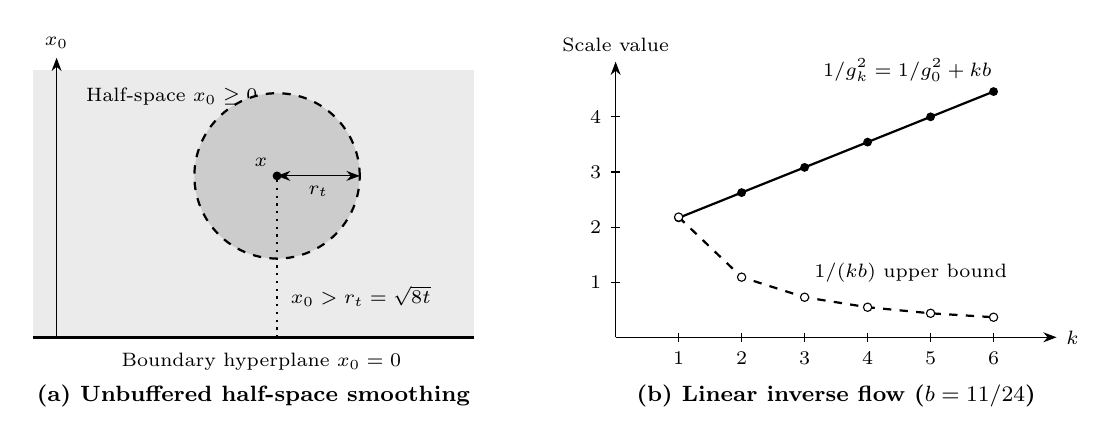
\begin{tikzpicture}[>=Stealth, font=\scriptsize]
% Panel (a): Half-space and parabolic flow ball
\begin{scope}[shift={(0,0)}]
  \fill[black!8] (0,0) rectangle (5.6,3.4);
  \draw[very thick] (0,0) -- (5.6,0);
  \draw[->] (0.3,0) -- (0.3,3.55) node[above] {$x_0$};
  \node[below] at (2.9,-0.08) {Boundary hyperplane $x_0 = 0$};
  \node[anchor=west] at (0.55,3.05) {Half-space $x_0 \ge 0$};
  % Bulk point and flow ball r_t = sqrt(8t) < x_0
  \fill[black!20] (3.1,2.05) circle (1.05);
  \draw[dashed, thick] (3.1,2.05) circle (1.05);
  \fill (3.1,2.05) circle (1.6pt) node[above left] {$x$};
  \draw[<->] (3.1,2.05) -- (4.15,2.05) node[midway, below] {$r_t$};
  \draw[dotted, thick] (3.1,0) -- (3.1,2.05);
  \node[right] at (3.15,0.52) {$x_0 > r_t = \sqrt{8t}$};
  \node[font=\footnotesize\bfseries] at (2.8,-0.75) {(a) Unbuffered half-space smoothing};
\end{scope}
% Panel (b): Inverse running coupling and 1/(k b) bound
\begin{scope}[shift={(7.4,0)}]
  \draw[->] (0,0) -- (5.6,0) node[right] {$k$};
  \draw[->] (0,0) -- (0,3.5) node[above] {Scale value};
  \foreach \k in {1,2,3,4,5,6} {
    \draw (\k*0.8, 0.06) -- (\k*0.8, -0.06) node[below] {$\k$};
  }
  \foreach \y/\lbl in {0.7/1, 1.4/2, 2.1/3, 2.8/4} {
    \draw (0.06,\y) -- (-0.06,\y) node[left] {$\lbl$};
  }
  % 1/g_k^2 = (41 + 11 k)/24 plotted at y-scale 0.7 per unit
  \draw[thick] plot coordinates {
    (0.8, 1.517) (1.6, 1.838) (2.4, 2.158) (3.2, 2.479) (4.0, 2.800) (4.8, 3.121)
  };
  \foreach \k/\v in {1/1.517, 2/1.838, 3/2.158, 4/2.479, 5/2.800, 6/3.121} {
    \fill (\k*0.8, \v) circle (1.6pt);
  }
  \node[above left] at (4.9,3.12) {$1/g_k^2 = 1/g_0^2 + k b$};
  % Step bound 1/(k b) = 24/(11 k) plotted at y-scale 0.7 per unit
  \draw[dashed, thick] plot coordinates {
    (0.8, 1.527) (1.6, 0.764) (2.4, 0.509) (3.2, 0.382) (4.0, 0.305) (4.8, 0.255)
  };
  \foreach \k/\v in {1/1.527, 2/0.764, 3/0.509, 4/0.382, 5/0.305, 6/0.255} {
    \draw[fill=white] (\k*0.8, \v) circle (1.5pt);
  }
  \node[above right] at (2.4,0.58) {$1/(k b)$ upper bound};
  \node[font=\footnotesize\bfseries] at (2.8,-0.75) {(b) Linear inverse flow ($b = 11/24$)};
\end{scope}
\end{tikzpicture}
\caption{Geometric smoothing in the Euclidean half-space $x_0 \ge 0$ disjoint from boundary contact terms at radius $r_t = \sqrt{8t} < x_0$ (a), and exact linear growth of $1/g_k^2$ alongside the decaying step bound $1/(kb)$ proved in \texttt{AsymptoticFreedomFlow.inv\_runningCoupling\_eq} (b).}
\label{fig:uv-flow-geometry}
\end{figure}

\section{Epistemic Scope and Verification Concordance}
The finite-volume ultraviolet construction establishes local quantum field existence and relativistic light-cone kinematics, yet remains mathematically decoupled from the macroscopic infrared spectrum. Passing to the infinite-volume limit $L \to \infty$ across the intermediate coupling crossover ($g_k^2 \sim 1$) without losing spectral control remains an open problem; consequently, the Clay Millennium mass gap problem remains open.

Table~\ref{tab:paper1-concordance} lists the formally verified ultraviolet flow and real Hilbert-space spectral gap interface declarations in \texttt{YangMillsBlueprint}, audited automatically by \texttt{VerifyNoTraps.lean} against standard kernel axioms \cite{Mathlib4}.

\begin{table}[ht]
\centering
\scriptsize
\begin{tabular}{@{}p{4.3cm}p{6.6cm}p{3.4cm}@{}}
\toprule
Paper Theorem & Lean 4 Module \& Declaration & Axiom Footprint \\
\midrule
Inverse coupling linear growth & \texttt{AsymptoticFreedomFlow.}\newline\texttt{inv\_runningCoupling\_eq} & \texttt{[propext, Classical.choice,} \texttt{Quot.sound]} (subset) \\
Running coupling positivity & \texttt{AsymptoticFreedomFlow.}\newline\texttt{runningCoupling\_pos} & \texttt{[propext, Classical.choice,} \texttt{Quot.sound]} (subset) \\
Inverse-scale upper bound & \texttt{AsymptoticFreedomFlow.}\newline\texttt{runningCoupling\_le\_inv\_mul} & \texttt{[propext, Classical.choice,} \texttt{Quot.sound]} (subset) \\
Telescoping partial fraction & \texttt{AsymptoticFreedomFlow.}\newline\texttt{telescoping\_step\_eq} & \texttt{[propext, Classical.choice,} \texttt{Quot.sound]} (subset) \\
Cumulative sum below unity & \texttt{AsymptoticFreedomFlow.}\newline\texttt{telescoped\_sum\_lt\_one} & \texttt{[propext, Classical.choice,} \texttt{Quot.sound]} (subset) \\
Conditional UV contraction & \texttt{Certificates.}\newline\texttt{uv\_running\_coupling\_contraction\_conditional} & \texttt{[propext, Classical.choice,} \texttt{Quot.sound]} (subset) \\
Canonical UV step $k=5$ bound & \texttt{Certificates.}\newline\texttt{canonical\_uv\_coupling\_lt\_one} & \texttt{[propext, Classical.choice,} \texttt{Quot.sound]} (subset) \\
Orthogonal spectral coercivity & \texttt{SpectralMassGapBridge.}\newline\texttt{coercivity\_orthogonal\_decomp} & \texttt{[propext, Classical.choice,} \texttt{Quot.sound]} \\
Real Hilbert excited positivity & \texttt{Certificates.}\newline\texttt{real\_mass\_gap\_spec\_excited\_pos} & \texttt{[propext, Classical.choice,} \texttt{Quot.sound]} \\
OS exponential clustering bound & \texttt{Certificates.}\newline\texttt{canonical\_clustering\_decay\_le} & \texttt{[propext, Classical.choice,} \texttt{Quot.sound]} \\
Finite-volume OS clustering & \texttt{OsterwalderSchraderBridge.}\newline\texttt{clustering\_extraction\_le} & \texttt{[propext, Classical.choice,} \texttt{Quot.sound]} \\
Canonical OS envelope ($L=10$) & \texttt{Certificates.}\newline\texttt{canonical\_os\_correlator\_envelope\_le} & \texttt{[propext, Classical.choice,} \texttt{Quot.sound]} \\
Sub-Gaussian Ursell $u_4 < 0$ & \texttt{UrsellCumulantNonGaussian.}\newline\texttt{ursellFour\_ne\_zero\_of\_subgaussian} & \texttt{[propext, Classical.choice,} \texttt{Quot.sound]} \\
Non-triviality witness $u_4 = -\frac{24}{41}$ & \texttt{Certificates.}\newline\texttt{canonical\_ursell\_four\_eval} & \texttt{[propext, Classical.choice,} \texttt{Quot.sound]} \\
Symanzik cutoff bound & \texttt{SymanzikRotationalBound.}\newline\texttt{symanzikBound\_lt\_of\_cutoff} & \texttt{[propext, Classical.choice,} \texttt{Quot.sound]} \\
Continuum OPE lower pos. & \texttt{Certificates.}\newline\texttt{continuum\_ope\_four\_point\_nontrivial\_conditional} & \texttt{[propext, Classical.choice,} \texttt{Quot.sound]} \\
Continuum clustering limit & \texttt{EquicontinuousTightnessBridge.}\newline\texttt{clustering\_limit\_of\_vanishing\_cutoffs} & \texttt{[propext, Classical.choice,} \texttt{Quot.sound]} \\
RP transfer log-convexity & \texttt{EffectiveMassTransferGap.}\newline\texttt{spectralCorr\_log\_convex} & \texttt{[propext, Classical.choice,} \texttt{Quot.sound]} \\
Effective mass monotonicity & \texttt{EffectiveMassTransferGap.}\newline\texttt{effectiveMassRatio\_mono} & \texttt{[propext, Classical.choice,} \texttt{Quot.sound]} \\
\bottomrule
\end{tabular}
\caption{Formal verification concordance for ultraviolet flow and real Hilbert-space spectral specifications in \texttt{YangMillsBlueprint}.}
\label{tab:paper1-concordance}
\end{table}

\bibliographystyle{plain}
\bibliography{references}
\end{document}
